% Technical report: electrode impedance with and without VR headsets,
% BrainAccess MINI (8 ch), MIDI (16 ch) and MAXI (32 ch).
% All numbers are generated by processing/impedance/impedance_over_time.ipynb
% and pulled in via \input below -- re-run the pipeline, then rebuild:
%   processing/impedance/run_pipeline.sh
\documentclass[11pt,a4paper]{article}
\usepackage[margin=2.2cm]{geometry}
\usepackage[T1]{fontenc}
\usepackage{lmodern}
\usepackage{graphicx}
\usepackage{booktabs}
\usepackage{amsmath}
\usepackage{caption}
\usepackage{enumitem}
\usepackage{xurl}
\usepackage[hidelinks]{hyperref}
\captionsetup{font=small,labelfont=bf}
\setlist{itemsep=2pt,topsep=4pt}
\setlength{\parindent}{0pt}
\setlength{\parskip}{5pt}
\setlength{\emergencystretch}{3em}
\graphicspath{{../figures/}}
% figures never taller than the page
\newcommand{\fig}[1]{\includegraphics[width=\textwidth,height=0.86\textheight,keepaspectratio]{#1}}

% Generated by processing/impedance/impedance_over_time.ipynb on 2026-11-06. Do not edit by hand.
% Group: impedance-S001-BA_MINI_8ch; sources: impedance-S001-NoVR-BA_MINI_8ch.csv, impedance-S001-HTC-BA_MINI_8ch.csv, impedance-S001-MetaQuest-BA_MINI_8ch.csv
\newcommand{\impNChannels}{8}
\newcommand{\impFs}{250}
\newcommand{\impDevice}{BA\_MINI\_8ch}
\newcommand{\impSession}{S001}
\newcommand{\impUnit}{k$\Omega$}
\newcommand{\impWindows}{1, 5, 15, 30}
\newcommand{\impRefWindow}{5}
\newcommand{\impEdge}{10}
\newcommand{\impTolPct}{10}
\newcommand{\impTolFrac}{0.1}
\newcommand{\impTolAbs}{10}
\newcommand{\impRunDate}{2026-11-06}
\newcommand{\impSubject}{sub-1}
\newcommand{\impDurNoVR}{154}
\newcommand{\impNSamplesNoVR}{38406}
\newcommand{\impMedMedNoVR}{87}
\newcommand{\impMedMinNoVR}{51}
\newcommand{\impMedMaxNoVR}{152}
\newcommand{\impMedMinChNoVR}{P4}
\newcommand{\impMedMaxChNoVR}{F4}
\newcommand{\impInitMedNoVR}{96}
\newcommand{\impFinalMedNoVR}{86}
\newcommand{\impNDecreaseNoVR}{5}
\newcommand{\impNIncreaseNoVR}{1}
\newcommand{\impSettleMedNoVR}{119}
\newcommand{\impSettleMaxNoVR}{142}
\newcommand{\impSettleMaxChNoVR}{P3}
\newcommand{\impMaxNoVR}{1784}
\newcommand{\impMaxChNoVR}{F4}
\newcommand{\impAboveMaxPctNoVR}{23.5}
\newcommand{\impAboveMaxChNoVR}{F4}
\newcommand{\impDropChNoVR}{F4}
\newcommand{\impDropInitNoVR}{1119}
\newcommand{\impDropFinalNoVR}{149}
\newcommand{\impDropSettleNoVR}{127}
\newcommand{\impNSettledSixtyNoVR}{2}
\newcommand{\impResidNoVRWone}{0.1}
\newcommand{\impSmoothMaxNoVRWone}{1147}
\newcommand{\impSlopeNoVRWone}{\ensuremath{-3.3}}
\newcommand{\impSlopeAbsMaxNoVRWone}{230.5}
\newcommand{\impResidNoVRWfive}{1.8}
\newcommand{\impSmoothMaxNoVRWfive}{1140}
\newcommand{\impSlopeNoVRWfive}{\ensuremath{-3.5}}
\newcommand{\impSlopeAbsMaxNoVRWfive}{249.4}
\newcommand{\impResidNoVRWonefive}{3.3}
\newcommand{\impSmoothMaxNoVRWonefive}{1132}
\newcommand{\impSlopeNoVRWonefive}{\ensuremath{-3.5}}
\newcommand{\impSlopeAbsMaxNoVRWonefive}{256.0}
\newcommand{\impResidNoVRWthreezero}{5.8}
\newcommand{\impSmoothMaxNoVRWthreezero}{1132}
\newcommand{\impSlopeNoVRWthreezero}{\ensuremath{-3.3}}
\newcommand{\impSlopeAbsMaxNoVRWthreezero}{309.0}
\newcommand{\impDurHTC}{156}
\newcommand{\impNSamplesHTC}{39000}
\newcommand{\impMedMedHTC}{83}
\newcommand{\impMedMinHTC}{14}
\newcommand{\impMedMaxHTC}{226}
\newcommand{\impMedMinChHTC}{O2}
\newcommand{\impMedMaxChHTC}{P3}
\newcommand{\impInitMedHTC}{112}
\newcommand{\impFinalMedHTC}{76}
\newcommand{\impNDecreaseHTC}{5}
\newcommand{\impNIncreaseHTC}{2}
\newcommand{\impSettleMedHTC}{35}
\newcommand{\impSettleMaxHTC}{120}
\newcommand{\impSettleMaxChHTC}{F3}
\newcommand{\impMaxHTC}{8288}
\newcommand{\impMaxChHTC}{F3}
\newcommand{\impAboveMaxPctHTC}{10.8}
\newcommand{\impAboveMaxChHTC}{F4}
\newcommand{\impDropChHTC}{P3}
\newcommand{\impDropInitHTC}{378}
\newcommand{\impDropFinalHTC}{92}
\newcommand{\impDropSettleHTC}{99}
\newcommand{\impNSettledSixtyHTC}{5}
\newcommand{\impResidHTCWone}{0.0}
\newcommand{\impSmoothMaxHTCWone}{428}
\newcommand{\impSlopeHTCWone}{\ensuremath{-4.1}}
\newcommand{\impSlopeAbsMaxHTCWone}{121.7}
\newcommand{\impResidHTCWfive}{1.4}
\newcommand{\impSmoothMaxHTCWfive}{428}
\newcommand{\impSlopeHTCWfive}{\ensuremath{-4.1}}
\newcommand{\impSlopeAbsMaxHTCWfive}{124.0}
\newcommand{\impResidHTCWonefive}{2.0}
\newcommand{\impSmoothMaxHTCWonefive}{414}
\newcommand{\impSlopeHTCWonefive}{\ensuremath{-4.4}}
\newcommand{\impSlopeAbsMaxHTCWonefive}{140.0}
\newcommand{\impResidHTCWthreezero}{2.2}
\newcommand{\impSmoothMaxHTCWthreezero}{385}
\newcommand{\impSlopeHTCWthreezero}{\ensuremath{-4.5}}
\newcommand{\impSlopeAbsMaxHTCWthreezero}{144.1}
\newcommand{\impDurMetaQuest}{168}
\newcommand{\impNSamplesMetaQuest}{42000}
\newcommand{\impMedMedMetaQuest}{83}
\newcommand{\impMedMinMetaQuest}{27}
\newcommand{\impMedMaxMetaQuest}{225}
\newcommand{\impMedMinChMetaQuest}{O1}
\newcommand{\impMedMaxChMetaQuest}{C3}
\newcommand{\impInitMedMetaQuest}{86}
\newcommand{\impFinalMedMetaQuest}{92}
\newcommand{\impNDecreaseMetaQuest}{5}
\newcommand{\impNIncreaseMetaQuest}{1}
\newcommand{\impSettleMedMetaQuest}{119}
\newcommand{\impSettleMaxMetaQuest}{149}
\newcommand{\impSettleMaxChMetaQuest}{F4}
\newcommand{\impMaxMetaQuest}{4357}
\newcommand{\impMaxChMetaQuest}{F4}
\newcommand{\impAboveMaxPctMetaQuest}{1.4}
\newcommand{\impAboveMaxChMetaQuest}{F4}
\newcommand{\impDropChMetaQuest}{C3}
\newcommand{\impDropInitMetaQuest}{337}
\newcommand{\impDropFinalMetaQuest}{96}
\newcommand{\impDropSettleMetaQuest}{118}
\newcommand{\impNSettledSixtyMetaQuest}{2}
\newcommand{\impResidMetaQuestWone}{0.0}
\newcommand{\impSmoothMaxMetaQuestWone}{4357}
\newcommand{\impSlopeMetaQuestWone}{\ensuremath{-5.8}}
\newcommand{\impSlopeAbsMaxMetaQuestWone}{106.7}
\newcommand{\impResidMetaQuestWfive}{1.2}
\newcommand{\impSmoothMaxMetaQuestWfive}{344}
\newcommand{\impSlopeMetaQuestWfive}{\ensuremath{-5.9}}
\newcommand{\impSlopeAbsMaxMetaQuestWfive}{108.2}
\newcommand{\impResidMetaQuestWonefive}{1.3}
\newcommand{\impSmoothMaxMetaQuestWonefive}{337}
\newcommand{\impSlopeMetaQuestWonefive}{\ensuremath{-6.6}}
\newcommand{\impSlopeAbsMaxMetaQuestWonefive}{114.0}
\newcommand{\impResidMetaQuestWthreezero}{1.6}
\newcommand{\impSmoothMaxMetaQuestWthreezero}{334}
\newcommand{\impSlopeMetaQuestWthreezero}{\ensuremath{-7.9}}
\newcommand{\impSlopeAbsMaxMetaQuestWthreezero}{125.9}
\newcommand{\impFriedmanStat}{2.25}
\newcommand{\impFriedmanP}{0.325}
\newcommand{\impWilcoxonHTCStat}{15}
\newcommand{\impWilcoxonHTCP}{0.742}
\newcommand{\impWilcoxonHTCDiff}{\ensuremath{-10}}
\newcommand{\impWilcoxonMetaQuestStat}{17}
\newcommand{\impWilcoxonMetaQuestP}{0.945}
\newcommand{\impWilcoxonMetaQuestDiff}{\ensuremath{-11}}

% Generated by processing/impedance/impedance_over_time.ipynb on 2026-11-06. Do not edit by hand.
% Group: impedance-S001-BA_MIDI_16ch; sources: impedance-S001-NoVR-BA_MIDI_16ch.csv, impedance-S001-HTC-BA_MIDI_16ch.csv, impedance-S001-MetaQuest-BA_MIDI_16ch.csv
\providecommand{\impUnit}{k$\Omega$}
\providecommand{\impWindows}{1, 5, 15, 30}
\providecommand{\impRefWindow}{5}
\providecommand{\impEdge}{10}
\providecommand{\impTolPct}{10}
\providecommand{\impTolFrac}{0.1}
\providecommand{\impTolAbs}{10}
\providecommand{\impRunDate}{2026-11-06}
\providecommand{\impSession}{S001}
\providecommand{\impMaxWindow}{30}
\providecommand{\impHighZ}{500}
\newcommand{\impMIDINChannels}{16}
\newcommand{\impMIDIChannels}{F7, F3, Fz, F4, F8, C3, Cz, C4, P7, P3, Pz, P4, P8, O1, Oz, O2}
\newcommand{\impMIDIFs}{250}
\newcommand{\impMIDIDevice}{BA\_MIDI\_16ch}
\newcommand{\impMIDISubject}{sub-1}
\newcommand{\impMIDIOrder}{No~VR, Meta~Quest, HTC~Vive}
\newcommand{\impMIDISpan}{33}
\newcommand{\impMIDIOffsetNoVR}{0}
\newcommand{\impMIDIMedFsevenNoVR}{406}
\newcommand{\impMIDIMedFthreeNoVR}{58}
\newcommand{\impMIDIMedFzNoVR}{255}
\newcommand{\impMIDIMedFfourNoVR}{71}
\newcommand{\impMIDIMedFeightNoVR}{86}
\newcommand{\impMIDIMedCthreeNoVR}{85}
\newcommand{\impMIDIMedCzNoVR}{75}
\newcommand{\impMIDIMedCfourNoVR}{1272}
\newcommand{\impMIDIMedPsevenNoVR}{50}
\newcommand{\impMIDIMedPthreeNoVR}{102}
\newcommand{\impMIDIMedPzNoVR}{69}
\newcommand{\impMIDIMedPfourNoVR}{102}
\newcommand{\impMIDIMedPeightNoVR}{65}
\newcommand{\impMIDIMedOoneNoVR}{84}
\newcommand{\impMIDIMedOzNoVR}{91}
\newcommand{\impMIDIMedOtwoNoVR}{63}
\newcommand{\impMIDIDurNoVR}{149}
\newcommand{\impMIDINSamplesNoVR}{37200}
\newcommand{\impMIDIMedMedNoVR}{84}
\newcommand{\impMIDIMedMinNoVR}{50}
\newcommand{\impMIDIMedMaxNoVR}{1272}
\newcommand{\impMIDIMedMinChNoVR}{P7}
\newcommand{\impMIDIMedMaxChNoVR}{C4}
\newcommand{\impMIDIInitMedNoVR}{80}
\newcommand{\impMIDIFinalMedNoVR}{82}
\newcommand{\impMIDINDecreaseNoVR}{4}
\newcommand{\impMIDINIncreaseNoVR}{6}
\newcommand{\impMIDISettleMedNoVR}{57}
\newcommand{\impMIDISettleMaxNoVR}{149}
\newcommand{\impMIDISettleMaxChNoVR}{P3}
\newcommand{\impMIDINSettledSixtyNoVR}{8}
\newcommand{\impMIDINHighNoVR}{1}
\newcommand{\impMIDIHighChNoVR}{C4}
\newcommand{\impMIDIMaxNoVR}{1345}
\newcommand{\impMIDIMaxChNoVR}{C4}
\newcommand{\impMIDIAboveMaxPctNoVR}{0.0}
\newcommand{\impMIDIAboveMaxChNoVR}{F7}
\newcommand{\impMIDIDropChNoVR}{F7}
\newcommand{\impMIDIDropInitNoVR}{524}
\newcommand{\impMIDIDropFinalNoVR}{362}
\newcommand{\impMIDIDropSettleNoVR}{107}
\newcommand{\impMIDIResidNoVRWone}{0.0}
\newcommand{\impMIDISmoothMaxNoVRWone}{1345}
\newcommand{\impMIDISlopeNoVRWone}{\ensuremath{+3.2}}
\newcommand{\impMIDISlopeAbsMaxNoVRWone}{48.7}
\newcommand{\impMIDINWinNoVRWone}{148}
\newcommand{\impMIDIResidNoVRWfive}{1.2}
\newcommand{\impMIDISmoothMaxNoVRWfive}{1345}
\newcommand{\impMIDISlopeNoVRWfive}{\ensuremath{+3.2}}
\newcommand{\impMIDISlopeAbsMaxNoVRWfive}{48.0}
\newcommand{\impMIDINWinNoVRWfive}{29}
\newcommand{\impMIDIResidNoVRWonefive}{1.9}
\newcommand{\impMIDISmoothMaxNoVRWonefive}{1315}
\newcommand{\impMIDISlopeNoVRWonefive}{\ensuremath{+3.4}}
\newcommand{\impMIDISlopeAbsMaxNoVRWonefive}{48.3}
\newcommand{\impMIDINWinNoVRWonefive}{9}
\newcommand{\impMIDIResidNoVRWthreezero}{2.1}
\newcommand{\impMIDISmoothMaxNoVRWthreezero}{1297}
\newcommand{\impMIDISlopeNoVRWthreezero}{\ensuremath{+3.0}}
\newcommand{\impMIDISlopeAbsMaxNoVRWthreezero}{61.7}
\newcommand{\impMIDINWinNoVRWthreezero}{4}
\newcommand{\impMIDIOffsetHTC}{33}
\newcommand{\impMIDIMedFsevenHTC}{162}
\newcommand{\impMIDIMedFthreeHTC}{151}
\newcommand{\impMIDIMedFzHTC}{19}
\newcommand{\impMIDIMedFfourHTC}{212}
\newcommand{\impMIDIMedFeightHTC}{52}
\newcommand{\impMIDIMedCthreeHTC}{185}
\newcommand{\impMIDIMedCzHTC}{27}
\newcommand{\impMIDIMedCfourHTC}{1218}
\newcommand{\impMIDIMedPsevenHTC}{192}
\newcommand{\impMIDIMedPthreeHTC}{158}
\newcommand{\impMIDIMedPzHTC}{23}
\newcommand{\impMIDIMedPfourHTC}{164}
\newcommand{\impMIDIMedPeightHTC}{98}
\newcommand{\impMIDIMedOoneHTC}{52}
\newcommand{\impMIDIMedOzHTC}{47}
\newcommand{\impMIDIMedOtwoHTC}{47}
\newcommand{\impMIDIDurHTC}{155}
\newcommand{\impMIDINSamplesHTC}{38800}
\newcommand{\impMIDIMedMedHTC}{124}
\newcommand{\impMIDIMedMinHTC}{19}
\newcommand{\impMIDIMedMaxHTC}{1218}
\newcommand{\impMIDIMedMinChHTC}{Fz}
\newcommand{\impMIDIMedMaxChHTC}{C4}
\newcommand{\impMIDIInitMedHTC}{108}
\newcommand{\impMIDIFinalMedHTC}{128}
\newcommand{\impMIDINDecreaseHTC}{5}
\newcommand{\impMIDINIncreaseHTC}{4}
\newcommand{\impMIDISettleMedHTC}{65}
\newcommand{\impMIDISettleMaxHTC}{155}
\newcommand{\impMIDISettleMaxChHTC}{C4}
\newcommand{\impMIDINSettledSixtyHTC}{6}
\newcommand{\impMIDINHighHTC}{1}
\newcommand{\impMIDIHighChHTC}{C4}
\newcommand{\impMIDIMaxHTC}{1350}
\newcommand{\impMIDIMaxChHTC}{C4}
\newcommand{\impMIDIAboveMaxPctHTC}{0.0}
\newcommand{\impMIDIAboveMaxChHTC}{F7}
\newcommand{\impMIDIDropChHTC}{C4}
\newcommand{\impMIDIDropInitHTC}{1261}
\newcommand{\impMIDIDropFinalHTC}{1059}
\newcommand{\impMIDIDropSettleHTC}{155}
\newcommand{\impMIDIResidHTCWone}{0.0}
\newcommand{\impMIDISmoothMaxHTCWone}{1350}
\newcommand{\impMIDISlopeHTCWone}{\ensuremath{+1.2}}
\newcommand{\impMIDISlopeAbsMaxHTCWone}{50.0}
\newcommand{\impMIDINWinHTCWone}{155}
\newcommand{\impMIDIResidHTCWfive}{1.6}
\newcommand{\impMIDISmoothMaxHTCWfive}{1322}
\newcommand{\impMIDISlopeHTCWfive}{\ensuremath{+1.2}}
\newcommand{\impMIDISlopeAbsMaxHTCWfive}{49.8}
\newcommand{\impMIDINWinHTCWfive}{31}
\newcommand{\impMIDIResidHTCWonefive}{2.4}
\newcommand{\impMIDISmoothMaxHTCWonefive}{1308}
\newcommand{\impMIDISlopeHTCWonefive}{\ensuremath{+0.8}}
\newcommand{\impMIDISlopeAbsMaxHTCWonefive}{58.0}
\newcommand{\impMIDINWinHTCWonefive}{10}
\newcommand{\impMIDIResidHTCWthreezero}{2.8}
\newcommand{\impMIDISmoothMaxHTCWthreezero}{1281}
\newcommand{\impMIDISlopeHTCWthreezero}{\ensuremath{+1.2}}
\newcommand{\impMIDISlopeAbsMaxHTCWthreezero}{54.8}
\newcommand{\impMIDINWinHTCWthreezero}{5}
\newcommand{\impMIDIOffsetMetaQuest}{27}
\newcommand{\impMIDIMedFsevenMetaQuest}{142}
\newcommand{\impMIDIMedFthreeMetaQuest}{145}
\newcommand{\impMIDIMedFzMetaQuest}{19}
\newcommand{\impMIDIMedFfourMetaQuest}{150}
\newcommand{\impMIDIMedFeightMetaQuest}{91}
\newcommand{\impMIDIMedCthreeMetaQuest}{121}
\newcommand{\impMIDIMedCzMetaQuest}{23}
\newcommand{\impMIDIMedCfourMetaQuest}{1287}
\newcommand{\impMIDIMedPsevenMetaQuest}{18}
\newcommand{\impMIDIMedPthreeMetaQuest}{88}
\newcommand{\impMIDIMedPzMetaQuest}{28}
\newcommand{\impMIDIMedPfourMetaQuest}{105}
\newcommand{\impMIDIMedPeightMetaQuest}{17}
\newcommand{\impMIDIMedOoneMetaQuest}{16}
\newcommand{\impMIDIMedOzMetaQuest}{34}
\newcommand{\impMIDIMedOtwoMetaQuest}{19}
\newcommand{\impMIDIDurMetaQuest}{154}
\newcommand{\impMIDINSamplesMetaQuest}{38400}
\newcommand{\impMIDIMedMedMetaQuest}{61}
\newcommand{\impMIDIMedMinMetaQuest}{16}
\newcommand{\impMIDIMedMaxMetaQuest}{1287}
\newcommand{\impMIDIMedMinChMetaQuest}{O1}
\newcommand{\impMIDIMedMaxChMetaQuest}{C4}
\newcommand{\impMIDIInitMedMetaQuest}{58}
\newcommand{\impMIDIFinalMedMetaQuest}{54}
\newcommand{\impMIDINDecreaseMetaQuest}{1}
\newcommand{\impMIDINIncreaseMetaQuest}{9}
\newcommand{\impMIDISettleMedMetaQuest}{0}
\newcommand{\impMIDISettleMaxMetaQuest}{139}
\newcommand{\impMIDISettleMaxChMetaQuest}{F8}
\newcommand{\impMIDINSettledSixtyMetaQuest}{11}
\newcommand{\impMIDINHighMetaQuest}{1}
\newcommand{\impMIDIHighChMetaQuest}{C4}
\newcommand{\impMIDIMaxMetaQuest}{1355}
\newcommand{\impMIDIMaxChMetaQuest}{C4}
\newcommand{\impMIDIAboveMaxPctMetaQuest}{0.0}
\newcommand{\impMIDIAboveMaxChMetaQuest}{F7}
\newcommand{\impMIDIDropChMetaQuest}{F8}
\newcommand{\impMIDIDropInitMetaQuest}{82}
\newcommand{\impMIDIDropFinalMetaQuest}{70}
\newcommand{\impMIDIDropSettleMetaQuest}{139}
\newcommand{\impMIDIResidMetaQuestWone}{0.0}
\newcommand{\impMIDISmoothMaxMetaQuestWone}{1355}
\newcommand{\impMIDISlopeMetaQuestWone}{\ensuremath{+2.1}}
\newcommand{\impMIDISlopeAbsMaxMetaQuestWone}{9.4}
\newcommand{\impMIDINWinMetaQuestWone}{153}
\newcommand{\impMIDIResidMetaQuestWfive}{1.0}
\newcommand{\impMIDISmoothMaxMetaQuestWfive}{1346}
\newcommand{\impMIDISlopeMetaQuestWfive}{\ensuremath{+1.8}}
\newcommand{\impMIDISlopeAbsMaxMetaQuestWfive}{9.3}
\newcommand{\impMIDINWinMetaQuestWfive}{30}
\newcommand{\impMIDIResidMetaQuestWonefive}{1.4}
\newcommand{\impMIDISmoothMaxMetaQuestWonefive}{1341}
\newcommand{\impMIDISlopeMetaQuestWonefive}{\ensuremath{+1.7}}
\newcommand{\impMIDISlopeAbsMaxMetaQuestWonefive}{9.0}
\newcommand{\impMIDINWinMetaQuestWonefive}{10}
\newcommand{\impMIDIResidMetaQuestWthreezero}{1.5}
\newcommand{\impMIDISmoothMaxMetaQuestWthreezero}{1315}
\newcommand{\impMIDISlopeMetaQuestWthreezero}{\ensuremath{+2.0}}
\newcommand{\impMIDISlopeAbsMaxMetaQuestWthreezero}{12.2}
\newcommand{\impMIDINWinMetaQuestWthreezero}{5}
\newcommand{\impMIDIFriedmanStat}{4.03}
\newcommand{\impMIDIFriedmanP}{0.133}
\newcommand{\impMIDIWilcoxonHTCStat}{64}
\newcommand{\impMIDIWilcoxonHTCP}{0.860}
\newcommand{\impMIDIWilcoxonHTCDiff}{\ensuremath{-24}}
\newcommand{\impMIDIWilcoxonMetaQuestStat}{40}
\newcommand{\impMIDIWilcoxonMetaQuestP}{0.159}
\newcommand{\impMIDIWilcoxonMetaQuestDiff}{\ensuremath{-36}}

% Generated by processing/impedance/impedance_over_time.ipynb on 2026-11-06. Do not edit by hand.
% Group: impedance-S001-BA_MAXI_32ch; sources: impedance-S001-NoVR-BA_MAXI_32ch.csv, impedance-S001-HTC-BA_MAXI_32ch.csv, impedance-S001-MetaQuest-BA_MAXI_32ch.csv
\providecommand{\impUnit}{k$\Omega$}
\providecommand{\impWindows}{1, 5, 15, 30}
\providecommand{\impRefWindow}{5}
\providecommand{\impEdge}{10}
\providecommand{\impTolPct}{10}
\providecommand{\impTolFrac}{0.1}
\providecommand{\impTolAbs}{10}
\providecommand{\impRunDate}{2026-11-06}
\providecommand{\impSession}{S001}
\providecommand{\impMaxWindow}{30}
\providecommand{\impHighZ}{500}
\newcommand{\impMAXINChannels}{32}
\newcommand{\impMAXIChannels}{AF3, AFz, AF4, F7, F3, Fz, F4, F8, FC5, FC1, FC2, FC6, C3, Cz, C4, T7, T8, CP5, CP1, CP2, CP6, P7, P3, Pz, P4, P8, PO3, POz, PO4, O1, Oz, O2}
\newcommand{\impMAXIFs}{250}
\newcommand{\impMAXIDevice}{BA\_MAXI\_32ch}
\newcommand{\impMAXISubject}{sub-1}
\newcommand{\impMAXIOrder}{No~VR, HTC~Vive, Meta~Quest}
\newcommand{\impMAXISpan}{10}
\newcommand{\impMAXIOffsetNoVR}{0}
\newcommand{\impMAXIMedAFthreeNoVR}{51}
\newcommand{\impMAXIMedAFzNoVR}{56}
\newcommand{\impMAXIMedAFfourNoVR}{34}
\newcommand{\impMAXIMedFsevenNoVR}{629}
\newcommand{\impMAXIMedFthreeNoVR}{36}
\newcommand{\impMAXIMedFzNoVR}{264}
\newcommand{\impMAXIMedFfourNoVR}{237}
\newcommand{\impMAXIMedFeightNoVR}{59}
\newcommand{\impMAXIMedFCfiveNoVR}{287}
\newcommand{\impMAXIMedFConeNoVR}{447}
\newcommand{\impMAXIMedFCtwoNoVR}{1434}
\newcommand{\impMAXIMedFCsixNoVR}{552}
\newcommand{\impMAXIMedCthreeNoVR}{391}
\newcommand{\impMAXIMedCzNoVR}{138}
\newcommand{\impMAXIMedCfourNoVR}{115}
\newcommand{\impMAXIMedTsevenNoVR}{86}
\newcommand{\impMAXIMedTeightNoVR}{115}
\newcommand{\impMAXIMedCPfiveNoVR}{77}
\newcommand{\impMAXIMedCPoneNoVR}{43}
\newcommand{\impMAXIMedCPtwoNoVR}{96}
\newcommand{\impMAXIMedCPsixNoVR}{104}
\newcommand{\impMAXIMedPsevenNoVR}{72}
\newcommand{\impMAXIMedPthreeNoVR}{989}
\newcommand{\impMAXIMedPzNoVR}{221}
\newcommand{\impMAXIMedPfourNoVR}{683}
\newcommand{\impMAXIMedPeightNoVR}{109}
\newcommand{\impMAXIMedPOthreeNoVR}{442}
\newcommand{\impMAXIMedPOzNoVR}{723}
\newcommand{\impMAXIMedPOfourNoVR}{466}
\newcommand{\impMAXIMedOoneNoVR}{132}
\newcommand{\impMAXIMedOzNoVR}{70}
\newcommand{\impMAXIMedOtwoNoVR}{283}
\newcommand{\impMAXIDurNoVR}{141}
\newcommand{\impMAXINSamplesNoVR}{35200}
\newcommand{\impMAXIMedMedNoVR}{135}
\newcommand{\impMAXIMedMinNoVR}{34}
\newcommand{\impMAXIMedMaxNoVR}{1434}
\newcommand{\impMAXIMedMinChNoVR}{AF4}
\newcommand{\impMAXIMedMaxChNoVR}{FC2}
\newcommand{\impMAXIInitMedNoVR}{242}
\newcommand{\impMAXIFinalMedNoVR}{121}
\newcommand{\impMAXINDecreaseNoVR}{21}
\newcommand{\impMAXINIncreaseNoVR}{5}
\newcommand{\impMAXISettleMedNoVR}{93}
\newcommand{\impMAXISettleMaxNoVR}{141}
\newcommand{\impMAXISettleMaxChNoVR}{Fz}
\newcommand{\impMAXINSettledSixtyNoVR}{6}
\newcommand{\impMAXINHighNoVR}{6}
\newcommand{\impMAXIHighChNoVR}{FC2, P3, POz, P4, F7, FC6}
\newcommand{\impMAXIMaxNoVR}{1602}
\newcommand{\impMAXIMaxChNoVR}{P3}
\newcommand{\impMAXIAboveMaxPctNoVR}{13.6}
\newcommand{\impMAXIAboveMaxChNoVR}{CP2}
\newcommand{\impMAXIDropChNoVR}{PO4}
\newcommand{\impMAXIDropInitNoVR}{1202}
\newcommand{\impMAXIDropFinalNoVR}{396}
\newcommand{\impMAXIDropSettleNoVR}{99}
\newcommand{\impMAXIResidNoVRWone}{0.0}
\newcommand{\impMAXISmoothMaxNoVRWone}{1565}
\newcommand{\impMAXISlopeNoVRWone}{\ensuremath{-30.4}}
\newcommand{\impMAXISlopeAbsMaxNoVRWone}{286.6}
\newcommand{\impMAXINWinNoVRWone}{140}
\newcommand{\impMAXIResidNoVRWfive}{0.0}
\newcommand{\impMAXISmoothMaxNoVRWfive}{1565}
\newcommand{\impMAXISlopeNoVRWfive}{\ensuremath{-31.6}}
\newcommand{\impMAXISlopeAbsMaxNoVRWfive}{283.4}
\newcommand{\impMAXINWinNoVRWfive}{28}
\newcommand{\impMAXIResidNoVRWonefive}{3.9}
\newcommand{\impMAXISmoothMaxNoVRWonefive}{1540}
\newcommand{\impMAXISlopeNoVRWonefive}{\ensuremath{-30.7}}
\newcommand{\impMAXISlopeAbsMaxNoVRWonefive}{312.2}
\newcommand{\impMAXINWinNoVRWonefive}{9}
\newcommand{\impMAXIResidNoVRWthreezero}{6.5}
\newcommand{\impMAXISmoothMaxNoVRWthreezero}{1520}
\newcommand{\impMAXISlopeNoVRWthreezero}{\ensuremath{-48.2}}
\newcommand{\impMAXISlopeAbsMaxNoVRWthreezero}{438.0}
\newcommand{\impMAXINWinNoVRWthreezero}{4}
\newcommand{\impMAXIOffsetHTC}{5}
\newcommand{\impMAXIMedAFthreeHTC}{29}
\newcommand{\impMAXIMedAFzHTC}{13}
\newcommand{\impMAXIMedAFfourHTC}{27}
\newcommand{\impMAXIMedFsevenHTC}{244}
\newcommand{\impMAXIMedFthreeHTC}{41}
\newcommand{\impMAXIMedFzHTC}{33}
\newcommand{\impMAXIMedFfourHTC}{114}
\newcommand{\impMAXIMedFeightHTC}{43}
\newcommand{\impMAXIMedFCfiveHTC}{314}
\newcommand{\impMAXIMedFConeHTC}{182}
\newcommand{\impMAXIMedFCtwoHTC}{372}
\newcommand{\impMAXIMedFCsixHTC}{336}
\newcommand{\impMAXIMedCthreeHTC}{198}
\newcommand{\impMAXIMedCzHTC}{34}
\newcommand{\impMAXIMedCfourHTC}{157}
\newcommand{\impMAXIMedTsevenHTC}{98}
\newcommand{\impMAXIMedTeightHTC}{135}
\newcommand{\impMAXIMedCPfiveHTC}{73}
\newcommand{\impMAXIMedCPoneHTC}{45}
\newcommand{\impMAXIMedCPtwoHTC}{47}
\newcommand{\impMAXIMedCPsixHTC}{105}
\newcommand{\impMAXIMedPsevenHTC}{73}
\newcommand{\impMAXIMedPthreeHTC}{261}
\newcommand{\impMAXIMedPzHTC}{74}
\newcommand{\impMAXIMedPfourHTC}{307}
\newcommand{\impMAXIMedPeightHTC}{81}
\newcommand{\impMAXIMedPOthreeHTC}{595}
\newcommand{\impMAXIMedPOzHTC}{260}
\newcommand{\impMAXIMedPOfourHTC}{460}
\newcommand{\impMAXIMedOoneHTC}{30}
\newcommand{\impMAXIMedOzHTC}{36}
\newcommand{\impMAXIMedOtwoHTC}{48}
\newcommand{\impMAXIDurHTC}{150}
\newcommand{\impMAXINSamplesHTC}{37600}
\newcommand{\impMAXIMedMedHTC}{90}
\newcommand{\impMAXIMedMinHTC}{13}
\newcommand{\impMAXIMedMaxHTC}{595}
\newcommand{\impMAXIMedMinChHTC}{AFz}
\newcommand{\impMAXIMedMaxChHTC}{PO3}
\newcommand{\impMAXIInitMedHTC}{122}
\newcommand{\impMAXIFinalMedHTC}{92}
\newcommand{\impMAXINDecreaseHTC}{18}
\newcommand{\impMAXINIncreaseHTC}{3}
\newcommand{\impMAXISettleMedHTC}{43}
\newcommand{\impMAXISettleMaxHTC}{144}
\newcommand{\impMAXISettleMaxChHTC}{F4}
\newcommand{\impMAXINSettledSixtyHTC}{18}
\newcommand{\impMAXINHighHTC}{1}
\newcommand{\impMAXIHighChHTC}{PO3}
\newcommand{\impMAXIMaxHTC}{1347}
\newcommand{\impMAXIMaxChHTC}{FC2}
\newcommand{\impMAXIAboveMaxPctHTC}{12.8}
\newcommand{\impMAXIAboveMaxChHTC}{Pz}
\newcommand{\impMAXIDropChHTC}{FC2}
\newcommand{\impMAXIDropInitHTC}{927}
\newcommand{\impMAXIDropFinalHTC}{267}
\newcommand{\impMAXIDropSettleHTC}{134}
\newcommand{\impMAXIResidHTCWone}{0.0}
\newcommand{\impMAXISmoothMaxHTCWone}{965}
\newcommand{\impMAXISlopeHTCWone}{\ensuremath{-4.3}}
\newcommand{\impMAXISlopeAbsMaxHTCWone}{168.5}
\newcommand{\impMAXINWinHTCWone}{150}
\newcommand{\impMAXIResidHTCWfive}{0.0}
\newcommand{\impMAXISmoothMaxHTCWfive}{965}
\newcommand{\impMAXISlopeHTCWfive}{\ensuremath{-4.4}}
\newcommand{\impMAXISlopeAbsMaxHTCWfive}{174.0}
\newcommand{\impMAXINWinHTCWfive}{30}
\newcommand{\impMAXIResidHTCWonefive}{2.0}
\newcommand{\impMAXISmoothMaxHTCWonefive}{927}
\newcommand{\impMAXISlopeHTCWonefive}{\ensuremath{-5.7}}
\newcommand{\impMAXISlopeAbsMaxHTCWonefive}{180.0}
\newcommand{\impMAXINWinHTCWonefive}{10}
\newcommand{\impMAXIResidHTCWthreezero}{2.4}
\newcommand{\impMAXISmoothMaxHTCWthreezero}{841}
\newcommand{\impMAXISlopeHTCWthreezero}{\ensuremath{-5.6}}
\newcommand{\impMAXISlopeAbsMaxHTCWthreezero}{164.0}
\newcommand{\impMAXINWinHTCWthreezero}{5}
\newcommand{\impMAXIOffsetMetaQuest}{10}
\newcommand{\impMAXIMedAFthreeMetaQuest}{40}
\newcommand{\impMAXIMedAFzMetaQuest}{19}
\newcommand{\impMAXIMedAFfourMetaQuest}{34}
\newcommand{\impMAXIMedFsevenMetaQuest}{331}
\newcommand{\impMAXIMedFthreeMetaQuest}{37}
\newcommand{\impMAXIMedFzMetaQuest}{37}
\newcommand{\impMAXIMedFfourMetaQuest}{153}
\newcommand{\impMAXIMedFeightMetaQuest}{45}
\newcommand{\impMAXIMedFCfiveMetaQuest}{294}
\newcommand{\impMAXIMedFConeMetaQuest}{375}
\newcommand{\impMAXIMedFCtwoMetaQuest}{322}
\newcommand{\impMAXIMedFCsixMetaQuest}{670}
\newcommand{\impMAXIMedCthreeMetaQuest}{364}
\newcommand{\impMAXIMedCzMetaQuest}{43}
\newcommand{\impMAXIMedCfourMetaQuest}{220}
\newcommand{\impMAXIMedTsevenMetaQuest}{76}
\newcommand{\impMAXIMedTeightMetaQuest}{124}
\newcommand{\impMAXIMedCPfiveMetaQuest}{43}
\newcommand{\impMAXIMedCPoneMetaQuest}{44}
\newcommand{\impMAXIMedCPtwoMetaQuest}{39}
\newcommand{\impMAXIMedCPsixMetaQuest}{120}
\newcommand{\impMAXIMedPsevenMetaQuest}{60}
\newcommand{\impMAXIMedPthreeMetaQuest}{424}
\newcommand{\impMAXIMedPzMetaQuest}{145}
\newcommand{\impMAXIMedPfourMetaQuest}{248}
\newcommand{\impMAXIMedPeightMetaQuest}{25}
\newcommand{\impMAXIMedPOthreeMetaQuest}{136}
\newcommand{\impMAXIMedPOzMetaQuest}{297}
\newcommand{\impMAXIMedPOfourMetaQuest}{231}
\newcommand{\impMAXIMedOoneMetaQuest}{32}
\newcommand{\impMAXIMedOzMetaQuest}{49}
\newcommand{\impMAXIMedOtwoMetaQuest}{45}
\newcommand{\impMAXIDurMetaQuest}{157}
\newcommand{\impMAXINSamplesMetaQuest}{39200}
\newcommand{\impMAXIMedMedMetaQuest}{98}
\newcommand{\impMAXIMedMinMetaQuest}{19}
\newcommand{\impMAXIMedMaxMetaQuest}{670}
\newcommand{\impMAXIMedMinChMetaQuest}{AFz}
\newcommand{\impMAXIMedMaxChMetaQuest}{FC6}
\newcommand{\impMAXIInitMedMetaQuest}{102}
\newcommand{\impMAXIFinalMedMetaQuest}{95}
\newcommand{\impMAXINDecreaseMetaQuest}{19}
\newcommand{\impMAXINIncreaseMetaQuest}{6}
\newcommand{\impMAXISettleMedMetaQuest}{13}
\newcommand{\impMAXISettleMaxMetaQuest}{138}
\newcommand{\impMAXISettleMaxChMetaQuest}{FC2}
\newcommand{\impMAXINSettledSixtyMetaQuest}{21}
\newcommand{\impMAXINHighMetaQuest}{1}
\newcommand{\impMAXIHighChMetaQuest}{FC6}
\newcommand{\impMAXIMaxMetaQuest}{779}
\newcommand{\impMAXIMaxChMetaQuest}{FC6}
\newcommand{\impMAXIAboveMaxPctMetaQuest}{2.1}
\newcommand{\impMAXIAboveMaxChMetaQuest}{Cz}
\newcommand{\impMAXIDropChMetaQuest}{PO4}
\newcommand{\impMAXIDropInitMetaQuest}{513}
\newcommand{\impMAXIDropFinalMetaQuest}{182}
\newcommand{\impMAXIDropSettleMetaQuest}{122}
\newcommand{\impMAXIResidMetaQuestWone}{0.0}
\newcommand{\impMAXISmoothMaxMetaQuestWone}{779}
\newcommand{\impMAXISlopeMetaQuestWone}{\ensuremath{-3.9}}
\newcommand{\impMAXISlopeAbsMaxMetaQuestWone}{85.4}
\newcommand{\impMAXINWinMetaQuestWone}{156}
\newcommand{\impMAXIResidMetaQuestWfive}{0.0}
\newcommand{\impMAXISmoothMaxMetaQuestWfive}{779}
\newcommand{\impMAXISlopeMetaQuestWfive}{\ensuremath{-3.7}}
\newcommand{\impMAXISlopeAbsMaxMetaQuestWfive}{88.0}
\newcommand{\impMAXINWinMetaQuestWfive}{31}
\newcommand{\impMAXIResidMetaQuestWonefive}{1.1}
\newcommand{\impMAXISmoothMaxMetaQuestWonefive}{778}
\newcommand{\impMAXISlopeMetaQuestWonefive}{\ensuremath{-3.8}}
\newcommand{\impMAXISlopeAbsMaxMetaQuestWonefive}{92.0}
\newcommand{\impMAXINWinMetaQuestWonefive}{10}
\newcommand{\impMAXIResidMetaQuestWthreezero}{1.5}
\newcommand{\impMAXISmoothMaxMetaQuestWthreezero}{769}
\newcommand{\impMAXISlopeMetaQuestWthreezero}{\ensuremath{-3.3}}
\newcommand{\impMAXISlopeAbsMaxMetaQuestWthreezero}{101.5}
\newcommand{\impMAXINWinMetaQuestWthreezero}{5}
\newcommand{\impMAXIFriedmanStat}{11.45}
\newcommand{\impMAXIFriedmanP}{0.003}
\newcommand{\impMAXIWilcoxonHTCStat}{78}
\newcommand{\impMAXIWilcoxonHTCP}{0.000}
\newcommand{\impMAXIWilcoxonHTCDiff}{\ensuremath{-38}}
\newcommand{\impMAXIWilcoxonMetaQuestStat}{62}
\newcommand{\impMAXIWilcoxonMetaQuestP}{0.000}
\newcommand{\impMAXIWilcoxonMetaQuestDiff}{\ensuremath{-47}}

% Generated by processing/impedance/impedance_over_time.ipynb on 2026-11-06. Do not edit by hand.
\newcommand{\impCommonChannels}{F3, F4, C3, C4, P3, P4, O1, O2}
\newcommand{\impNCommon}{8}
\newcommand{\impMAXICommonMedNoVR}{260}
\newcommand{\impMAXICommonMedHTC}{136}
\newcommand{\impMAXICommonMedMetaQuest}{186}
\newcommand{\impMIDICommonMedNoVR}{84}
\newcommand{\impMIDICommonMedHTC}{161}
\newcommand{\impMIDICommonMedMetaQuest}{113}
\newcommand{\impMINICommonMedNoVR}{87}
\newcommand{\impMINICommonMedHTC}{83}
\newcommand{\impMINICommonMedMetaQuest}{83}


\begin{document}

{\Large\bfseries Technical report: EEG electrode impedance under VR headsets}\par
\vspace{2pt}
{\large BrainAccess MINI (\impMININChannels{} ch), MIDI (\impMIDINChannels{} ch)
and MAXI (\impMAXINChannels{} ch) with HTC~Vive and Meta~Quest}\par
\vspace{8pt}
\begin{tabular}{@{}ll@{}}
Date: & \impRunDate \\
Prepared by: & EEG-VR-stats project \quad % TODO: name / contact
\\
Data: & 1 participant, session \impSession; 3 recordings per device (no VR, HTC, Meta~Quest) \\
\end{tabular}
\vspace{4pt}\hrule

\section{Summary}
\begin{itemize}
  \item \textbf{VR headsets did not raise impedance overall.} Median impedance
    across electrodes (no VR / HTC~Vive / Meta~Quest) was
    \impMINIMedMedNoVR{} / \impMINIMedMedHTC{} / \impMINIMedMedMetaQuest~\impUnit{} (MINI),
    \impMIDIMedMedNoVR{} / \impMIDIMedMedHTC{} / \impMIDIMedMedMetaQuest~\impUnit{} (MIDI) and
    \impMAXIMedMedNoVR{} / \impMAXIMedMedHTC{} / \impMAXIMedMedMetaQuest~\impUnit{} (MAXI).
    Only MAXI shows a systematic difference (lower with VR), but its no-VR
    recording was the first after fitting and impedance was still falling
    steeply (\impMAXISlopeNoVRWfive~\impUnit/min), so this most likely reflects
    settling rather than the headsets.
  \item \textbf{Midline electrodes were much lower under both VR headsets} on
    MIDI and MAXI (Fz \impMIDIMedFzNoVR\,\(\to\)\,\impMIDIMedFzHTC{} /
    \impMIDIMedFzMetaQuest~\impUnit{} on MIDI, \impMAXIMedFzNoVR\,\(\to\)\,\impMAXIMedFzHTC{} /
    \impMAXIMedFzMetaQuest~\impUnit{} on MAXI; HTC / Meta~Quest). Other
    electrodes changed in both directions.
  \item \textbf{Electrodes to check:} MIDI C4 was above 1000~\impUnit{} in every
    recording (\impMIDIMedCfourNoVR, \impMIDIMedCfourHTC, \impMIDIMedCfourMetaQuest~\impUnit).
    On MAXI, \impMAXINHighNoVR{} electrodes had a median above
    \impHighZ~\impUnit{} without VR (\impMAXIHighChNoVR).
  \item \textbf{Settling.} Impedance fell during the first minutes with MINI and
    especially MAXI; with MAXI only \impMAXINSettledSixtyNoVR{} of
    \impMAXINChannels{} electrodes were stable from 60~s onwards in the first
    (no-VR) recording. MIDI was stable from early on.
  \item \textbf{Short spikes} occurred with MINI (up to \impMINIMaxHTC~\impUnit)
    and in one MAXI recording (\impMAXIMaxHTC~\impUnit). \textbf{A 5-s rolling
    median} removes them and keeps real changes.
\end{itemize}

\section{Setup}
{\small
\begin{tabular}{@{}lp{0.23\textwidth}p{0.24\textwidth}p{0.29\textwidth}@{}}
\toprule
 & \textbf{MINI} & \textbf{MIDI} & \textbf{MAXI} \\
\midrule
Device & BrainAccess MINI & BrainAccess MIDI & BrainAccess MAXI \\
Electrodes (\(n\)) & \impMININChannels: \impMINIChannels & \impMIDINChannels: \impMIDIChannels & \impMAXINChannels: \impMAXIChannels \\
Sampling rate & \impMINIFs~Hz & \impMIDIFs~Hz & \impMAXIFs~Hz \\
Recording order & \impMINIOrder & \impMIDIOrder & \impMAXIOrder \\
Start (min)\textsuperscript{*} & 0 / \impMINIOffsetHTC{} / \impMINIOffsetMetaQuest &
   0 / \impMIDIOffsetHTC{} / \impMIDIOffsetMetaQuest & 0 / \impMAXIOffsetHTC{} / \impMAXIOffsetMetaQuest \\
Duration (s)\textsuperscript{*} & \impMINIDurNoVR{} / \impMINIDurHTC{} / \impMINIDurMetaQuest &
   \impMIDIDurNoVR{} / \impMIDIDurHTC{} / \impMIDIDurMetaQuest & \impMAXIDurNoVR{} / \impMAXIDurHTC{} / \impMAXIDurMetaQuest \\
\bottomrule
\end{tabular}\\[2pt]
\textsuperscript{*}no VR / HTC~Vive / Meta~Quest; start relative to the first recording with that device.}

All recordings were made in impedance mode with dry electrodes and one
participant (\impMINISubject) on the same day; each device was fitted
separately, and the VR headset was worn over the EEG headset. Recordings were
exported from the acquisition software (SQLite) to CSV; dates, device serial
numbers and computer timestamps were removed. No data were excluded or
interpolated.

\section{Processing}
\begin{itemize}
  \item Each electrode's impedance was smoothed with a centred rolling median
    of \impWindows~s. The median ignores isolated spikes.
  \item \textbf{Initial / final impedance:} median of the first / last \impEdge~s.
  \item \textbf{Settling time:} last moment the \impRefWindow-s median was more
    than \(\max(\impTolPct\%,\ \impTolAbs~\text{\impUnit})\) away from the final value.
  \item \textbf{Trend:} robust (Theil--Sen) slope of the impedance over time, in \impUnit/min.
  \item \textbf{High impedance:} electrode median above \impHighZ~\impUnit{}
    (a reporting threshold, not a device specification).
\end{itemize}

\section{Results}
\subsection{Device overview}
On the \impNCommon{} electrodes present on all devices (\impCommonChannels),
median impedance without VR was similar for MINI and MIDI
(\impMINICommonMedNoVR{} and \impMIDICommonMedNoVR~\impUnit) and higher for
MAXI (\impMAXICommonMedNoVR~\impUnit); see Table~\ref{tab:devices}. Each
device was fitted separately, so this compares fittings as much as devices.

\begin{table}[htbp]
  \centering
  \caption{Median over electrodes of the per-electrode median impedance
  (\impUnit): on the \impNCommon{} common electrodes and on all electrodes of
  each device (number of electrodes in brackets).}
  \label{tab:devices}
  \small
  \begin{tabular}{lrrrrrr}
\toprule
 & \multicolumn{2}{c}{No VR} & \multicolumn{2}{c}{HTC Vive} & \multicolumn{2}{c}{Meta Quest} \\
\cmidrule(lr){2-3}\cmidrule(lr){4-5}\cmidrule(lr){6-7}
Device & common (8) & all & common (8) & all & common (8) & all \\
\midrule
BA\_MAXI\_32ch & 260 & 135 (32) & 136 & 90 (32) & 186 & 98 (32) \\
BA\_MIDI\_16ch & 84 & 84 (16) & 161 & 124 (16) & 113 & 61 (16) \\
BA\_MINI\_8ch & 87 & 87 (8) & 83 & 83 (8) & 83 & 83 (8) \\
\bottomrule
\end{tabular}

\end{table}

\subsection{MINI (\impMININChannels{} channels)}
\begin{itemize}
  \item Electrode medians ranged from \impMINIMedMinNoVR{} (\impMINIMedMinChNoVR) to
    \impMINIMedMaxNoVR~\impUnit{} (\impMINIMedMaxChNoVR) without VR,
    \impMINIMedMinHTC{} (\impMINIMedMinChHTC) to \impMINIMedMaxHTC~\impUnit{}
    (\impMINIMedMaxChHTC) with HTC and \impMINIMedMinMetaQuest{}
    (\impMINIMedMinChMetaQuest) to \impMINIMedMaxMetaQuest~\impUnit{}
    (\impMINIMedMaxChMetaQuest) with Meta~Quest; no consistent shift between
    conditions (Friedman \(p = \impMINIFriedmanP\)).
  \item Impedance fell by more than \impTolPct\% in \impMININDecreaseNoVR,
    \impMININDecreaseHTC{} and \impMININDecreaseMetaQuest{} of
    \impMININChannels{} electrodes (no VR, HTC, Meta~Quest), mostly in steps.
    Largest drops: \impMINIDropChNoVR{}
    \impMINIDropInitNoVR\,\(\to\)\,\impMINIDropFinalNoVR, \impMINIDropChHTC{}
    \impMINIDropInitHTC\,\(\to\)\,\impMINIDropFinalHTC, \impMINIDropChMetaQuest{}
    \impMINIDropInitMetaQuest\,\(\to\)\,\impMINIDropFinalMetaQuest~\impUnit.
  \item Median settling time \impMINISettleMedNoVR, \impMINISettleMedHTC{} and
    \impMINISettleMedMetaQuest~s; only \impMININSettledSixtyNoVR,
    \impMININSettledSixtyHTC{} and \impMININSettledSixtyMetaQuest{} electrodes
    were stable from 60~s onwards.
  \item Spikes up to \impMINIMaxHTC~\impUnit{} (\impMINIMaxChHTC, HTC) and
    \impMINIMaxMetaQuest~\impUnit{} (\impMINIMaxChMetaQuest, Meta~Quest).
\end{itemize}

\begin{figure}[htbp]
  \centering
  \fig{impedance_conditions_impedance-S001-BA_MINI_8ch.pdf}
  \caption{MINI: impedance (\impUnit, log scale) per electrode, \impRefWindow-s
  rolling median, one recording per condition (\impMINIFs~Hz;
  \(n = \impMININSamplesNoVR, \impMININSamplesHTC, \impMININSamplesMetaQuest\) samples).}
  \label{fig:mini}
\end{figure}

\begin{table}[htbp]
  \centering
  \caption{MINI: impedance per electrode (\impUnit): median [interquartile
  range], initial\,\(\to\)\,final value, and settling time (s).}
  \label{tab:mini}
  \footnotesize\setlength{\tabcolsep}{3.5pt}
  \resizebox{\textwidth}{!}{\begin{tabular}{lrrrrrrrrr}
\toprule
 & \multicolumn{3}{c}{No VR} & \multicolumn{3}{c}{HTC Vive} & \multicolumn{3}{c}{Meta Quest} \\
\cmidrule(lr){2-4}\cmidrule(lr){5-7}\cmidrule(lr){8-10}
Ch. & median [IQR] & init.\,$\to$\,final & settle (s) & median [IQR] & init.\,$\to$\,final & settle (s) & median [IQR] & init.\,$\to$\,final & settle (s) \\
\midrule
F3 & 103 [94--127] & 902\,$\to$\,93 & 70 & 102 [87--227] & 248\,$\to$\,101 & 120 & 87 [79--100] & 81\,$\to$\,105 & 120 \\
F4 & 152 [128--431] & 1119\,$\to$\,149 & 127 & 119 [113--344] & 385\,$\to$\,115 & 75 & 206 [151--270] & 284\,$\to$\,206 & 149 \\
C3 & 76 [74--79] & 81\,$\to$\,78 & 0 & 141 [139--143] & 150\,$\to$\,146 & 0 & 225 [105--316] & 337\,$\to$\,96 & 118 \\
C4 & 102 [100--106] & 120\,$\to$\,98 & 111 & 64 [61--67] & 74\,$\to$\,59 & 22 & 66 [63--86] & 85\,$\to$\,65 & 70 \\
P3 & 98 [95--126] & 109\,$\to$\,237 & 142 & 226 [94--267] & 378\,$\to$\,92 & 99 & 92 [78--170] & 212\,$\to$\,94 & 144 \\
P4 & 51 [48--52] & 83\,$\to$\,45 & 15 & 50 [47--54] & 48\,$\to$\,57 & 48 & 79 [77--84] & 87\,$\to$\,89 & 125 \\
O1 & 51 [48--61] & 68\,$\to$\,60 & 137 & 31 [29--33] & 36\,$\to$\,28 & 0 & 27 [25--30] & 36\,$\to$\,25 & 7 \\
O2 & 63 [55--69] & 64\,$\to$\,65 & 127 & 14 [13--15] & 13\,$\to$\,17 & 0 & 28 [26--29] & 28\,$\to$\,28 & 0 \\
\bottomrule
\end{tabular}
}
\end{table}

\subsection{MIDI (\impMIDINChannels{} channels)}
\begin{itemize}
  \item Electrode medians ranged from \impMIDIMedMinNoVR{} (\impMIDIMedMinChNoVR) to
    \impMIDIMedMaxNoVR~\impUnit{} (\impMIDIMedMaxChNoVR) without VR,
    \impMIDIMedMinHTC{} (\impMIDIMedMinChHTC) to \impMIDIMedMaxHTC~\impUnit{}
    (\impMIDIMedMaxChHTC) with HTC and \impMIDIMedMinMetaQuest{}
    (\impMIDIMedMinChMetaQuest) to \impMIDIMedMaxMetaQuest~\impUnit{}
    (\impMIDIMedMaxChMetaQuest) with Meta~Quest; no consistent shift between
    conditions (Friedman \(p = \impMIDIFriedmanP\)).
  \item \textbf{Midline electrodes} were much lower with both VR headsets than
    without: Fz \impMIDIMedFzNoVR{} vs.\ \impMIDIMedFzHTC{} (HTC) and
    \impMIDIMedFzMetaQuest~\impUnit{} (Meta~Quest), Cz \impMIDIMedCzNoVR{} vs.\
    \impMIDIMedCzHTC{} and \impMIDIMedCzMetaQuest, Pz \impMIDIMedPzNoVR{} vs.\
    \impMIDIMedPzHTC{} and \impMIDIMedPzMetaQuest~\impUnit.
  \item \textbf{Lateral fronto-central electrodes} were higher with both
    headsets: F3 \impMIDIMedFthreeNoVR{} vs.\ \impMIDIMedFthreeHTC{} /
    \impMIDIMedFthreeMetaQuest, F4 \impMIDIMedFfourNoVR{} vs.\
    \impMIDIMedFfourHTC{} / \impMIDIMedFfourMetaQuest, C3
    \impMIDIMedCthreeNoVR{} vs.\ \impMIDIMedCthreeHTC{} /
    \impMIDIMedCthreeMetaQuest~\impUnit{} (HTC / Meta~Quest).
  \item \textbf{Posterior electrodes} were lowest with Meta~Quest (P7
    \impMIDIMedPsevenMetaQuest, P8 \impMIDIMedPeightMetaQuest, O1
    \impMIDIMedOoneMetaQuest, O2 \impMIDIMedOtwoMetaQuest~\impUnit), while P7
    was highest with HTC (\impMIDIMedPsevenHTC~\impUnit).
  \item \textbf{C4} stayed at \impMIDIMedCfourNoVR, \impMIDIMedCfourHTC{} and
    \impMIDIMedCfourMetaQuest~\impUnit{} in all three recordings. On MAXI,
    C4 was normal (\impMAXIMedCfourNoVR--\impMAXIMedCfourMetaQuest~\impUnit),
    which points to the MIDI electrode or its connector rather than the position.
  \item Impedance was stable: median settling time \impMIDISettleMedNoVR,
    \impMIDISettleMedHTC{} and \impMIDISettleMedMetaQuest~s;
    \impMIDINSettledSixtyNoVR, \impMIDINSettledSixtyHTC{} and
    \impMIDINSettledSixtyMetaQuest{} of \impMIDINChannels{} electrodes were
    stable from 60~s onwards. No spikes comparable to MINI occurred.
\end{itemize}

\begin{figure}[htbp]
  \centering
  \fig{impedance_conditions_impedance-S001-BA_MIDI_16ch.pdf}
  \caption{MIDI: impedance (\impUnit, log scale) per electrode, \impRefWindow-s
  rolling median, one recording per condition (\impMIDIFs~Hz;
  \(n = \impMIDINSamplesNoVR, \impMIDINSamplesHTC, \impMIDINSamplesMetaQuest\) samples).}
  \label{fig:midi}
\end{figure}

\begin{table}[htbp]
  \centering
  \caption{MIDI: impedance per electrode (\impUnit): median [interquartile
  range], initial\,\(\to\)\,final value, and settling time (s).}
  \label{tab:midi}
  \footnotesize\setlength{\tabcolsep}{3.5pt}
  \resizebox{\textwidth}{!}{\begin{tabular}{lrrrrrrrrr}
\toprule
 & \multicolumn{3}{c}{No VR} & \multicolumn{3}{c}{HTC Vive} & \multicolumn{3}{c}{Meta Quest} \\
\cmidrule(lr){2-4}\cmidrule(lr){5-7}\cmidrule(lr){8-10}
Ch. & median [IQR] & init.\,$\to$\,final & settle (s) & median [IQR] & init.\,$\to$\,final & settle (s) & median [IQR] & init.\,$\to$\,final & settle (s) \\
\midrule
F7 & 406 [398--440] & 524\,$\to$\,362 & 107 & 162 [160--163] & 161\,$\to$\,163 & 0 & 142 [139--144] & 138\,$\to$\,142 & 0 \\
F3 & 58 [55--60] & 55\,$\to$\,60 & 0 & 151 [149--156] & 154\,$\to$\,152 & 64 & 145 [143--148] & 143\,$\to$\,150 & 0 \\
Fz & 255 [246--296] & 332\,$\to$\,243 & 72 & 19 [18--22] & 17\,$\to$\,22 & 0 & 19 [18--20] & 19\,$\to$\,22 & 0 \\
F4 & 71 [63--76] & 55\,$\to$\,76 & 61 & 212 [207--219] & 238\,$\to$\,208 & 66 & 150 [145--155] & 148\,$\to$\,161 & 46 \\
F8 & 86 [83--89] & 111\,$\to$\,71 & 141 & 52 [48--56] & 45\,$\to$\,60 & 96 & 91 [87--93] & 82\,$\to$\,70 & 139 \\
C3 & 85 [81--89] & 77\,$\to$\,89 & 29 & 185 [161--190] & 164\,$\to$\,183 & 94 & 121 [117--124] & 116\,$\to$\,133 & 72 \\
Cz & 75 [71--82] & 79\,$\to$\,70 & 115 & 27 [25--29] & 26\,$\to$\,27 & 64 & 23 [22--25] & 24\,$\to$\,26 & 0 \\
C4 & 1272 [1230--1312] & 1253\,$\to$\,1278 & 0 & 1218 [1142--1279] & 1261\,$\to$\,1059 & 155 & 1287 [1247--1322] & 1312\,$\to$\,1330 & 0 \\
P7 & 50 [48--53] & 47\,$\to$\,52 & 0 & 192 [183--213] & 217\,$\to$\,176 & 94 & 18 [17--19] & 16\,$\to$\,29 & 126 \\
P3 & 102 [99--106] & 97\,$\to$\,105 & 149 & 158 [118--164] & 120\,$\to$\,155 & 94 & 88 [87--91] & 86\,$\to$\,107 & 139 \\
Pz & 69 [66--71] & 65\,$\to$\,72 & 32 & 23 [21--24] & 23\,$\to$\,24 & 0 & 28 [27--30] & 30\,$\to$\,31 & 0 \\
P4 & 102 [99--106] & 98\,$\to$\,107 & 77 & 164 [161--172] & 223\,$\to$\,161 & 67 & 105 [102--108] & 102\,$\to$\,115 & 69 \\
P8 & 65 [57--74] & 55\,$\to$\,71 & 139 & 98 [94--100] & 97\,$\to$\,103 & 54 & 17 [16--18] & 16\,$\to$\,19 & 0 \\
O1 & 84 [81--87] & 81\,$\to$\,88 & 35 & 52 [49--54] & 50\,$\to$\,52 & 0 & 16 [15--18] & 16\,$\to$\,19 & 0 \\
Oz & 91 [89--95] & 90\,$\to$\,96 & 53 & 47 [42--51] & 66\,$\to$\,40 & 34 & 34 [32--35] & 33\,$\to$\,37 & 0 \\
O2 & 63 [60--67] & 60\,$\to$\,68 & 34 & 47 [46--49] & 50\,$\to$\,45 & 67 & 19 [18--21] & 19\,$\to$\,21 & 0 \\
\bottomrule
\end{tabular}
}
\end{table}

\subsection{MAXI (\impMAXINChannels{} channels)}
\begin{itemize}
  \item Electrode medians ranged from \impMAXIMedMinNoVR{} (\impMAXIMedMinChNoVR) to
    \impMAXIMedMaxNoVR~\impUnit{} (\impMAXIMedMaxChNoVR) without VR,
    \impMAXIMedMinHTC{} (\impMAXIMedMinChHTC) to \impMAXIMedMaxHTC~\impUnit{}
    (\impMAXIMedMaxChHTC) with HTC and \impMAXIMedMinMetaQuest{}
    (\impMAXIMedMinChMetaQuest) to \impMAXIMedMaxMetaQuest~\impUnit{}
    (\impMAXIMedMaxChMetaQuest) with Meta~Quest. Impedance was lower in both VR
    recordings than in the no-VR recording (Friedman \(p = \impMAXIFriedmanP\)).
  \item \textbf{This difference is confounded with settling.} The no-VR
    recording came first and impedance was falling in
    \impMAXINDecreaseNoVR{} of \impMAXINChannels{} electrodes (median trend
    \impMAXISlopeNoVRWfive~\impUnit/min; median settling time
    \impMAXISettleMedNoVR~s; only \impMAXINSettledSixtyNoVR{} electrodes stable
    from 60~s). In the later VR recordings trends were small
    (\impMAXISlopeHTCWfive{} and \impMAXISlopeMetaQuestWfive~\impUnit/min) and
    \impMAXINSettledSixtyHTC{} and \impMAXINSettledSixtyMetaQuest{} electrodes
    were stable from 60~s.
  \item \textbf{Midline and occipital electrodes} were much lower with both VR
    headsets: Fz \impMAXIMedFzNoVR{} vs.\ \impMAXIMedFzHTC{} /
    \impMAXIMedFzMetaQuest, Cz \impMAXIMedCzNoVR{} vs.\ \impMAXIMedCzHTC{} /
    \impMAXIMedCzMetaQuest, O1 \impMAXIMedOoneNoVR{} vs.\ \impMAXIMedOoneHTC{} /
    \impMAXIMedOoneMetaQuest, O2 \impMAXIMedOtwoNoVR{} vs.\ \impMAXIMedOtwoHTC{} /
    \impMAXIMedOtwoMetaQuest~\impUnit{} (HTC / Meta~Quest).
  \item \textbf{High-impedance electrodes} (median above \impHighZ~\impUnit):
    \impMAXINHighNoVR{} without VR (\impMAXIHighChNoVR), \impMAXINHighHTC{}
    with HTC (\impMAXIHighChHTC) and \impMAXINHighMetaQuest{} with Meta~Quest
    (\impMAXIHighChMetaQuest). CP2 showed repeated short jumps without VR
    (Fig.~\ref{fig:maxi}), typical of intermittent contact.
  \item One spike up to \impMAXIMaxHTC~\impUnit{} (\impMAXIMaxChHTC, HTC); the
    highest 1-s median in that recording was \impMAXISmoothMaxHTCWone~\impUnit.
\end{itemize}

\begin{figure}[p]
  \centering
  \fig{impedance_conditions_impedance-S001-BA_MAXI_32ch.pdf}
  \caption{MAXI: impedance (\impUnit, log scale) per electrode, \impRefWindow-s
  rolling median, one recording per condition (\impMAXIFs~Hz;
  \(n = \impMAXINSamplesNoVR, \impMAXINSamplesHTC, \impMAXINSamplesMetaQuest\) samples).}
  \label{fig:maxi}
\end{figure}

\begin{table}[p]
  \centering
  \caption{MAXI: impedance per electrode (\impUnit): median [interquartile
  range], initial\,\(\to\)\,final value, and settling time (s).}
  \label{tab:maxi}
  \footnotesize\setlength{\tabcolsep}{3.5pt}
  \resizebox{\textwidth}{!}{\begin{tabular}{lrrrrrrrrr}
\toprule
 & \multicolumn{3}{c}{No VR} & \multicolumn{3}{c}{HTC Vive} & \multicolumn{3}{c}{Meta Quest} \\
\cmidrule(lr){2-4}\cmidrule(lr){5-7}\cmidrule(lr){8-10}
Ch. & median [IQR] & init.\,$\to$\,final & settle (s) & median [IQR] & init.\,$\to$\,final & settle (s) & median [IQR] & init.\,$\to$\,final & settle (s) \\
\midrule
AF3 & 51 [45--57] & 34\,$\to$\,43 & 134 & 29 [26--31] & 24\,$\to$\,32 & 0 & 40 [38--41] & 37\,$\to$\,42 & 0 \\
AFz & 56 [47--66] & 47\,$\to$\,36 & 125 & 13 [13--15] & 13\,$\to$\,15 & 64 & 19 [18--19] & 17\,$\to$\,19 & 0 \\
AF4 & 34 [32--36] & 29\,$\to$\,32 & 32 & 27 [24--30] & 20\,$\to$\,29 & 115 & 34 [32--35] & 30\,$\to$\,36 & 0 \\
F7 & 629 [551--745] & 930\,$\to$\,506 & 93 & 244 [240--252] & 270\,$\to$\,233 & 19 & 331 [328--333] & 321\,$\to$\,335 & 0 \\
F3 & 36 [33--40] & 38\,$\to$\,36 & 38 & 41 [39--43] & 45\,$\to$\,36 & 19 & 37 [35--39] & 42\,$\to$\,34 & 0 \\
Fz & 264 [226--354] & 208\,$\to$\,191 & 141 & 33 [29--44] & 112\,$\to$\,33 & 138 & 37 [37--39] & 38\,$\to$\,43 & 0 \\
F4 & 237 [219--254] & 160\,$\to$\,219 & 118 & 114 [111--119] & 131\,$\to$\,129 & 144 & 153 [151--156] & 159\,$\to$\,151 & 0 \\
F8 & 59 [55--62] & 61\,$\to$\,51 & 61 & 43 [42--44] & 45\,$\to$\,44 & 0 & 45 [44--47] & 44\,$\to$\,49 & 0 \\
FC5 & 287 [276--291] & 291\,$\to$\,275 & 13 & 314 [307--317] & 293\,$\to$\,320 & 3 & 294 [288--303] & 297\,$\to$\,279 & 61 \\
FC1 & 447 [404--497] & 497\,$\to$\,351 & 125 & 182 [174--206] & 284\,$\to$\,168 & 83 & 375 [341--390] & 432\,$\to$\,317 & 109 \\
FC2 & 1434 [1374--1494] & 1540\,$\to$\,1306 & 77 & 372 [314--558] & 927\,$\to$\,267 & 134 & 322 [299--378] & 519\,$\to$\,283 & 138 \\
FC6 & 552 [530--670] & 821\,$\to$\,494 & 83 & 336 [332--340] & 350\,$\to$\,311 & 80 & 670 [627--722] & 778\,$\to$\,610 & 80 \\
C3 & 391 [304--554] & 972\,$\to$\,275 & 109 & 198 [195--203] & 205\,$\to$\,204 & 0 & 364 [359--367] & 381\,$\to$\,358 & 0 \\
Cz & 138 [134--156] & 130\,$\to$\,130 & 74 & 34 [30--48] & 161\,$\to$\,27 & 61 & 43 [41--44] & 74\,$\to$\,43 & 10 \\
C4 & 115 [112--132] & 236\,$\to$\,112 & 51 & 157 [155--159] & 171\,$\to$\,161 & 0 & 220 [208--228] & 241\,$\to$\,199 & 86 \\
T7 & 86 [81--92] & 74\,$\to$\,89 & 29 & 98 [96--99] & 99\,$\to$\,100 & 0 & 76 [75--78] & 73\,$\to$\,83 & 83 \\
T8 & 115 [110--119] & 119\,$\to$\,109 & 61 & 135 [131--140] & 132\,$\to$\,139 & 0 & 124 [122--132] & 149\,$\to$\,123 & 29 \\
CP5 & 77 [70--108] & 167\,$\to$\,70 & 61 & 73 [72--76] & 94\,$\to$\,73 & 26 & 43 [41--44] & 47\,$\to$\,40 & 3 \\
CP1 & 43 [41--45] & 43\,$\to$\,39 & 13 & 45 [44--48] & 50\,$\to$\,45 & 0 & 44 [41--50] & 67\,$\to$\,37 & 51 \\
CP2 & 96 [69--155] & 130\,$\to$\,73 & 134 & 47 [41--56] & 84\,$\to$\,39 & 74 & 39 [36--42] & 48\,$\to$\,33 & 26 \\
CP6 & 104 [97--140] & 273\,$\to$\,98 & 118 & 105 [103--108] & 111\,$\to$\,108 & 0 & 120 [119--122] & 130\,$\to$\,119 & 3 \\
P7 & 72 [69--84] & 91\,$\to$\,77 & 131 & 73 [70--75] & 82\,$\to$\,77 & 6 & 60 [59--62] & 72\,$\to$\,62 & 3 \\
P3 & 989 [879--1193] & 1427\,$\to$\,813 & 96 & 261 [252--282] & 336\,$\to$\,244 & 58 & 424 [421--430] & 443\,$\to$\,421 & 0 \\
Pz & 221 [198--247] & 247\,$\to$\,193 & 80 & 74 [61--131] & 490\,$\to$\,55 & 106 & 145 [140--147] & 151\,$\to$\,131 & 83 \\
P4 & 683 [602--823] & 1131\,$\to$\,551 & 93 & 307 [298--331] & 368\,$\to$\,292 & 51 & 248 [246--249] & 247\,$\to$\,250 & 0 \\
P8 & 109 [103--152] & 274\,$\to$\,98 & 70 & 81 [79--83] & 88\,$\to$\,83 & 0 & 25 [23--30] & 25\,$\to$\,22 & 77 \\
PO3 & 442 [386--525] & 574\,$\to$\,359 & 90 & 595 [556--654] & 714\,$\to$\,523 & 93 & 136 [115--173] & 257\,$\to$\,107 & 106 \\
POz & 723 [653--788] & 850\,$\to$\,614 & 96 & 260 [230--343] & 678\,$\to$\,217 & 102 & 297 [290--304] & 329\,$\to$\,277 & 80 \\
PO4 & 466 [426--730] & 1202\,$\to$\,396 & 99 & 460 [453--477] & 584\,$\to$\,477 & 13 & 231 [200--300] & 513\,$\to$\,182 & 122 \\
O1 & 132 [116--200] & 373\,$\to$\,104 & 131 & 30 [27--39] & 51\,$\to$\,27 & 80 & 32 [31--33] & 39\,$\to$\,31 & 0 \\
Oz & 70 [58--82] & 62\,$\to$\,95 & 118 & 36 [31--49] & 69\,$\to$\,30 & 90 & 49 [46--52] & 68\,$\to$\,43 & 35 \\
O2 & 283 [259--401] & 870\,$\to$\,233 & 131 & 48 [47--56] & 78\,$\to$\,47 & 35 & 45 [44--47] & 63\,$\to$\,44 & 16 \\
\bottomrule
\end{tabular}
}
\end{table}

\subsection{Choice of smoothing window}
Rolling medians of all four lengths agree for most of the time and differ only
around spikes and short changes (Fig.~\ref{fig:windows} and
Appendix~\ref{app:figs}). Tables~\ref{tab:windows-mini}--\ref{tab:windows-maxi}
and Fig.~\ref{fig:sensitivity} summarise the effect:
\begin{itemize}
  \item For stable recordings the trend estimate barely depends on the window
    (1-s vs.\ 30-s: \impMINISlopeNoVRWone{} vs.\ \impMINISlopeNoVRWthreezero{}
    for MINI and \impMIDISlopeNoVRWone{} vs.\ \impMIDISlopeNoVRWthreezero~\impUnit/min
    for MIDI, no VR). For the steeply falling MAXI no-VR recording it changed
    from \impMAXISlopeNoVRWone{} to \impMAXISlopeNoVRWthreezero~\impUnit/min,
    the 30-s value resting on only \impMAXINWinNoVRWthreezero{} points; use
    windows of \(\leq\)15~s for trends over recordings of this length.
  \item With MINI, a 1-s window removed the HTC spike (\impMINIMaxHTC~\impUnit)
    but not the Meta~Quest excursion (\impMINIMaxMetaQuest~\impUnit); a 5-s
    window removed both.
  \item 15--30~s windows also remove genuine short changes, e.g.\ the brief rise
    of F4 at about 65~s in the MINI no-VR recording, visible only at 1 and 5~s.
\end{itemize}

\begin{figure}[htbp]
  \centering
  \fig{impedance_windows_impedance-S001-NoVR-BA_MINI_8ch.pdf}
  \caption{MINI, no-VR recording: raw impedance (grey) and rolling medians of
  \impWindows~s (light to dark blue). Log scale.}
  \label{fig:windows}
\end{figure}

\begin{figure}[htbp]
  \centering
  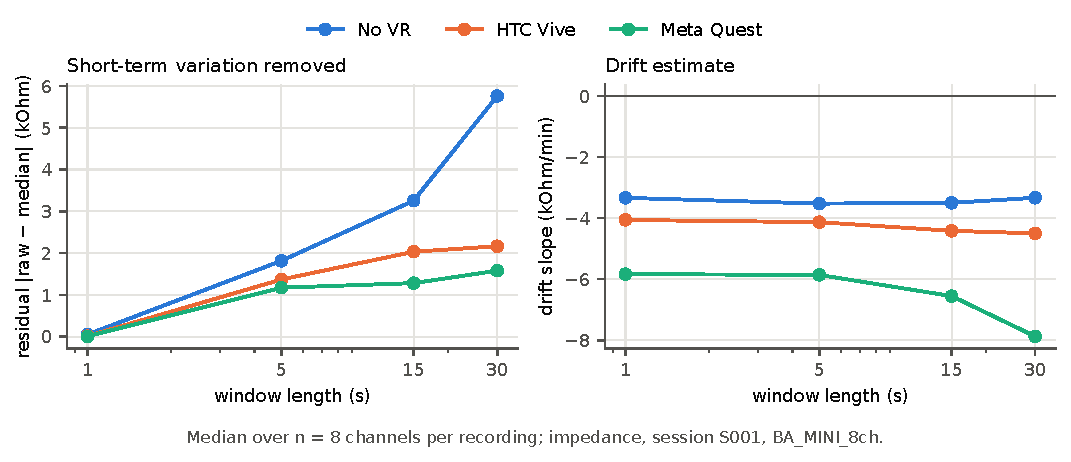
\includegraphics[width=0.92\textwidth]{impedance_window_sensitivity_impedance-S001-BA_MINI_8ch.pdf}\\[2pt]
  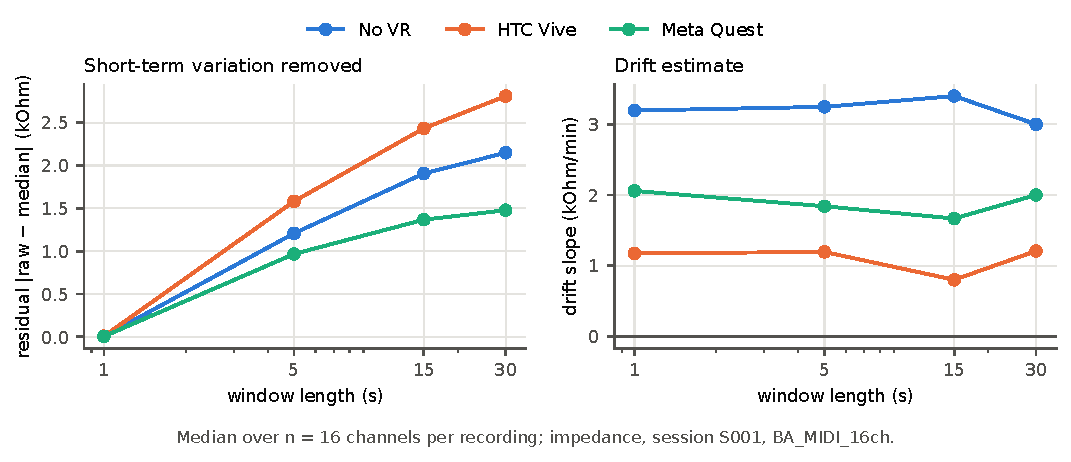
\includegraphics[width=0.92\textwidth]{impedance_window_sensitivity_impedance-S001-BA_MIDI_16ch.pdf}\\[2pt]
  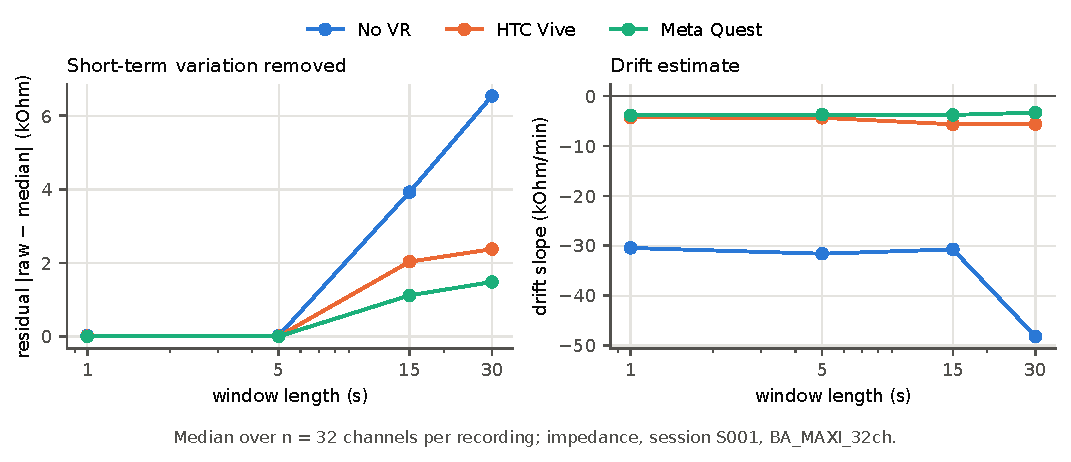
\includegraphics[width=0.92\textwidth]{impedance_window_sensitivity_impedance-S001-BA_MAXI_32ch.pdf}
  \caption{Effect of window length, MINI (top), MIDI (middle) and MAXI
  (bottom). Left: average difference between raw and smoothed impedance (what
  the window removes). Right: trend estimate. Median over electrodes per
  recording.}
  \label{fig:sensitivity}
\end{figure}

\begin{table}[htbp]
  \centering
  \caption{MINI, effect of window length: average removed variation (\impUnit)
  and trend (\impUnit/min), median over \impMININChannels{} electrodes.}
  \label{tab:windows-mini}
  \small
  \resizebox{\textwidth}{!}{\begin{tabular}{rrrrrrr}
\toprule
 & \multicolumn{2}{c}{No VR} & \multicolumn{2}{c}{HTC Vive} & \multicolumn{2}{c}{Meta Quest} \\
\cmidrule(lr){2-3}\cmidrule(lr){4-5}\cmidrule(lr){6-7}
Window (s) & resid. (k$\Omega$) & slope (k$\Omega$/min) & resid. (k$\Omega$) & slope (k$\Omega$/min) & resid. (k$\Omega$) & slope (k$\Omega$/min) \\
\midrule
1 & 0.1 & \ensuremath{-3.3} & 0.0 & \ensuremath{-4.1} & 0.0 & \ensuremath{-5.8} \\
5 & 1.8 & \ensuremath{-3.5} & 1.4 & \ensuremath{-4.1} & 1.2 & \ensuremath{-5.9} \\
15 & 3.3 & \ensuremath{-3.5} & 2.0 & \ensuremath{-4.4} & 1.3 & \ensuremath{-6.6} \\
30 & 5.8 & \ensuremath{-3.3} & 2.2 & \ensuremath{-4.5} & 1.6 & \ensuremath{-7.9} \\
\bottomrule
\end{tabular}
}
\end{table}

\begin{table}[htbp]
  \centering
  \caption{MIDI, effect of window length: average removed variation (\impUnit)
  and trend (\impUnit/min), median over \impMIDINChannels{} electrodes.}
  \label{tab:windows-midi}
  \small
  \resizebox{\textwidth}{!}{\begin{tabular}{rrrrrrr}
\toprule
 & \multicolumn{2}{c}{No VR} & \multicolumn{2}{c}{HTC Vive} & \multicolumn{2}{c}{Meta Quest} \\
\cmidrule(lr){2-3}\cmidrule(lr){4-5}\cmidrule(lr){6-7}
Window (s) & resid. (k$\Omega$) & slope (k$\Omega$/min) & resid. (k$\Omega$) & slope (k$\Omega$/min) & resid. (k$\Omega$) & slope (k$\Omega$/min) \\
\midrule
1 & 0.0 & \ensuremath{+3.2} & 0.0 & \ensuremath{+1.2} & 0.0 & \ensuremath{+2.1} \\
5 & 1.2 & \ensuremath{+3.2} & 1.6 & \ensuremath{+1.2} & 1.0 & \ensuremath{+1.8} \\
15 & 1.9 & \ensuremath{+3.4} & 2.4 & \ensuremath{+0.8} & 1.4 & \ensuremath{+1.7} \\
30 & 2.1 & \ensuremath{+3.0} & 2.8 & \ensuremath{+1.2} & 1.5 & \ensuremath{+2.0} \\
\bottomrule
\end{tabular}
}
\end{table}

\begin{table}[htbp]
  \centering
  \caption{MAXI, effect of window length: average removed variation (\impUnit)
  and trend (\impUnit/min), median over \impMAXINChannels{} electrodes.}
  \label{tab:windows-maxi}
  \small
  \resizebox{\textwidth}{!}{\begin{tabular}{rrrrrrr}
\toprule
 & \multicolumn{2}{c}{No VR} & \multicolumn{2}{c}{HTC Vive} & \multicolumn{2}{c}{Meta Quest} \\
\cmidrule(lr){2-3}\cmidrule(lr){4-5}\cmidrule(lr){6-7}
Window (s) & resid. (k$\Omega$) & slope (k$\Omega$/min) & resid. (k$\Omega$) & slope (k$\Omega$/min) & resid. (k$\Omega$) & slope (k$\Omega$/min) \\
\midrule
1 & 0.0 & \ensuremath{-30.4} & 0.0 & \ensuremath{-4.3} & 0.0 & \ensuremath{-3.9} \\
5 & 0.0 & \ensuremath{-31.6} & 0.0 & \ensuremath{-4.4} & 0.0 & \ensuremath{-3.7} \\
15 & 3.9 & \ensuremath{-30.7} & 2.0 & \ensuremath{-5.7} & 1.1 & \ensuremath{-3.8} \\
30 & 6.5 & \ensuremath{-48.2} & 2.4 & \ensuremath{-5.6} & 1.5 & \ensuremath{-3.3} \\
\bottomrule
\end{tabular}
}
\end{table}

\section{Recommendations}
\begin{enumerate}
  \item Display or log impedance with a \textbf{5-s rolling median}; use
    windows up to 15~s for reporting trends.
  \item \textbf{Check hardware/fit:} MIDI C4 (above 1000~\impUnit{} in every
    recording, normal on MAXI); on MAXI the electrodes above \impHighZ~\impUnit{}
    (\impMAXIHighChNoVR) and CP2 (intermittent contact).
  \item Allow a \textbf{settling period} after fitting the EEG headset and
    re-check impedance before recording. With MINI and MAXI, 2.5--3~minutes
    were not enough for all electrodes.
  \item Re-check impedance \textbf{after putting on the VR headset}: it changed
    individual electrodes in both directions (midline lower on MIDI and MAXI;
    some lateral electrodes higher), so a pre-VR check is not sufficient.
  \item For a fair VR comparison, \textbf{record a settled no-VR baseline} (or
    randomise the order of conditions); in this data set the no-VR recording
    always came first.
\end{enumerate}

\section{Limitations}
One participant, one recording per condition and device. Conditions were
recorded in a fixed order that differed between devices (MINI: \impMINIOrder;
MIDI: \impMIDIOrder; MAXI: \impMAXIOrder), always starting without VR, so
differences between conditions may also reflect time since fitting or
re-fitting of the headsets. Results should be confirmed with more participants
and a balanced order of conditions.

\clearpage
\appendix
\section{Window comparison, remaining recordings}\label{app:figs}
\begin{figure}[p]\centering
  \fig{impedance_windows_impedance-S001-HTC-BA_MINI_8ch.pdf}
  \caption{MINI, HTC~Vive; as Fig.~\ref{fig:windows}.}\end{figure}
\begin{figure}[p]\centering
  \fig{impedance_windows_impedance-S001-MetaQuest-BA_MINI_8ch.pdf}
  \caption{MINI, Meta~Quest; as Fig.~\ref{fig:windows}.}\end{figure}
\begin{figure}[p]\centering
  \fig{impedance_windows_impedance-S001-NoVR-BA_MIDI_16ch.pdf}
  \caption{MIDI, no VR; as Fig.~\ref{fig:windows}.}\end{figure}
\begin{figure}[p]\centering
  \fig{impedance_windows_impedance-S001-HTC-BA_MIDI_16ch.pdf}
  \caption{MIDI, HTC~Vive; as Fig.~\ref{fig:windows}.}\end{figure}
\begin{figure}[p]\centering
  \fig{impedance_windows_impedance-S001-MetaQuest-BA_MIDI_16ch.pdf}
  \caption{MIDI, Meta~Quest; as Fig.~\ref{fig:windows}.}\end{figure}
\begin{figure}[p]\centering
  \fig{impedance_windows_impedance-S001-NoVR-BA_MAXI_32ch.pdf}
  \caption{MAXI, no VR; as Fig.~\ref{fig:windows}.}\end{figure}
\begin{figure}[p]\centering
  \fig{impedance_windows_impedance-S001-HTC-BA_MAXI_32ch.pdf}
  \caption{MAXI, HTC~Vive; as Fig.~\ref{fig:windows}.}\end{figure}
\begin{figure}[p]\centering
  \fig{impedance_windows_impedance-S001-MetaQuest-BA_MAXI_32ch.pdf}
  \caption{MAXI, Meta~Quest; as Fig.~\ref{fig:windows}.}\end{figure}
\clearpage

\section{Data and reproducibility}
Generated by \nolinkurl{processing/impedance/impedance_over_time.ipynb} from
\nolinkurl{datafiles/impedance/impedance-S001-*-BA_*.csv} (MINI, MIDI, MAXI);
parameters and source checksums are in
\nolinkurl{outputs/impedance/impedance_provenance_impedance-S001-*.json}.
To regenerate: \nolinkurl{processing/impedance/run_pipeline.sh}.

\end{document}
